\chapter{Pairwise space and $M^2TML$ formalization}
\label{sec:unchapitre}
\minitoc


%\noindent Chapeau introductif
%\begin{itemize}
%	\item Le calcul d'une métrique implique toujours 2 individus. On va proposer un changement d'espace, un nouvel espace : la représentation par paire.
%	\item Le cadre : on suppose que l'on a p métriques.
%\end{itemize}

\fbox{  \parbox{0.9\textwidth}{
		In this chapter, we formalize the problem of the PhD. Our aim is to learn a metric that combines different modalities at different scales. The computation of a metric always implies a pair of samples. In this chapter, we propose to define a new space, the pairwise space in which a pair of time series is embedded as a vector described by the different metrics at different scales. Inspired from the Metric Learning framework, we transpose the metric learning problem in the pairwise space to propose a Multi-Modal and Multi-scale Time series Metric Learning framework for the classification and regression of time series.
	}  }

%---------------------------------------------------------------------------
\section{Pairwise space representation}
%\begin{itemize}
%	\item Changement de l'espace
%	\item Normalisation de l'espace des paires
%	\item Label des pairwise
%\end{itemize}

\noindent \textbf{Pairwise embedding} \\
Let  $d_1, ..., d_h ..., d_p$ be $p$ given dissimilarity metrics that allow to compare samples. The computation of a metric always takes into account a pair of samples. We introduce a new space representation referred as the pairwise space. In this new space, illustrated in Figure \ref{fig:PairwiseEmbedding}, a vector $\textbf{x}_{ij}$ represents a pair of samples $(\textbf{x}_i,\textbf{x}_j)$ described by the $p$ basics metrics $d_h$: $\textbf{x}_{ij}=[d_1(\textbf{x}_i,\textbf{x}_j), ..., d_p(\textbf{x}_i,\textbf{x}_j)]^T$.
%		\begin{equation*}		
%			\textbf{x}_{ij}
%			=
%			\begin{bmatrix}
%		        d_1(\textbf{x}_i,\textbf{x}_j) 	\\
%		        ... 			\\
%		       	d_p(\textbf{x}_i,\textbf{x}_j)
%		     \end{bmatrix}	    	     
%		\end{equation*}


\begin{figure}[h!]
	\begin{minipage}[b]{1.0\linewidth}
		\centering
		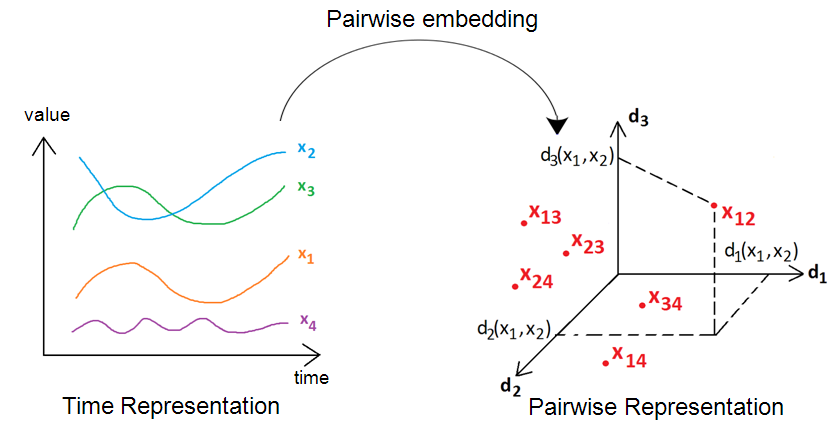
\includegraphics[width=0.8\linewidth]{images/PairwiseEmbedding}
	\end{minipage}
	\caption{Example of embedding of time series $\textbf{x}_i$ from the temporal space (left) into the pairwise space (right). In this example, a pair of time series $(\textbf{x}_1, \textbf{x}_2)$ is projected into the pairwise space as a vector $\textbf{x}_{12}$ described by $p=3$ basic metrics: $\textbf{x}_{12} = [d_1(\textbf{x}_1, \textbf{x}_2), d_2(\textbf{x}_1, \textbf{x}_2), d_3(\textbf{x}_1, \textbf{x}_2)]^T$.}
	\label{fig:PairwiseEmbedding}
\end{figure}

A combination function $D$ of the metrics $d_h$ can be seen as a function in this space. We propose in the following to use a linear combination of $d_h$: $D_w(\textbf{x}_i,\textbf{x}_j) = \sum_h w_h.d_h(\textbf{x}_i,\textbf{x}_j)$. Its pairwise notation is:
\begin{equation}
D_w(\textbf{x}_{ij})=\textbf{w}^T.\textbf{x}_{ij}
\end{equation}



\noindent \textbf{Pairwise label} \\
In classification problems, each pair $(\textbf{x}_i,\textbf{x}_j)$ is labeled:
\begin{equation}
	y_{ij} = 
	\left\{
	\begin{split}
	-1 \text{\quad if } y_i = y_j\\ 
	+1 \text{\quad if } y_i \neq y_j
	\end{split}
	\right.
\end{equation}
In regression problems, two approaches are possible. The first one aims to discretize by binning the label $y_i$ into $Q$ intervals as illustrated in Fig. ??. Each interval becomes a class which associated value can be set for example as the mean or median value of the interval. Then, the practitioner use the classification framework.

\missingfigure{Mettre une figure ici montrant la discretization. Faire 2 figures, la 1ère montre dans le domaine temporal et son équivalent en classe. La 2ème est une figure entrée/sortie}  

\noindent The second technic consider a tube of size $\epsilon$ around each value of $y_i$.

%---------------------------------------------------------------------------
\subsection{Interpretation of the pairwise space}
\begin{itemize}
	\item Proximity to the origin (les individus sont identiques)
	\item Proximity of 2 pairwise points in the pairwise space 
	\item Norm in the pairwise space
	\item Representation of combined metric in the pairwise space
\end{itemize}
%%% Local Variables: 
%%% mode: latex
%%% TeX-master: "../roque-phdthesis"
%%% End: 
If $\textbf{x}_{ij}=\textbf{0}$ then $\textbf{x}_{j}$ is identical to $\textbf{x}_{i}$ according to all metrics $d_h$.

%---------------------------------------------------------------------------
\subsection{Pros \& Cons}
\begin{itemize}
	\item perte de la classe initiale des individus. L'information qui nous reste est : les 2 individus sont de la même classe ou sont de classes différentes.
\end{itemize}



\section{$M^2TML$: LP optimization problem}
\begin{itemize}
	\item Formaliser le problème sous forme d'un problème d'optimisation sous contraintes
\end{itemize}

\section{$M^2TML$: QP optimization problem}
\begin{itemize}
	\item Passer de la forme LP (forme primale) et par transformation, arriver à la forme duale
	\item Montrer les similitudes avec la résolution SVM
	\item Montrer que l'on peut kerneliser la méthode
\end{itemize}


\section{$M^2TML$: SVM approximation}
\begin{itemize}
	\item Faire remarquer que le problème LP ressemble à un problème SVM
	\item Faire la démonstration de l'équivalence (ou mettre la démonstration en annexe).
	\item Expliquer les différences entre la résolution LP/QP et la résolution SVM. (ajout de sur-contraintes dans le problème SVM)
	\item Expliquer pourquoi on va préférer le cadre SVM. Expliquer mathématiquement et avec des interprétations géométriques. 
	\item Cadre connu
	\item Utilisation de librairie standard de Machine Learning
	\item Extension directe à l'apprentissage de métrique non linéaire grâce au kernel trick
\end{itemize}
